\section{GOAL-GAMYGDALA Interface}
Now that you have an understanding of how GOAL works and how GAMYGDALA works, it is possible to understand the architecture of the interface between the two, and the considerations that were made in the process of creating this architecture.
There are some significant differences between the way GOAL works and the way GAMYGDALA works. Understanding these differences is fundamental in the process of designing the interface between the two. After all, the goal of the interface is to cross these differences the best it can.

\subsection{Architecture overview}
The GOAL-GAMYGDALA interface architecture consists of three major parts: the Term Parser, which parses the terms into basic java values, the main interface, which is the interface from GOAL to global GAMYGDALA actions, and the agent interface, which is the interface from GOAL to agent-specific actions.

\subsubsection{Term Parser}
When a call is made in GOAL, this is done in the form of terms. Terms define the basic structure of a GOAL value, though the only current implementation is in Prolog. Since our GAMYGDALA port is in java, it expects basic java values, so we need to transform these Terms to primary values or lists. This is done by using a term parser.
We have used the Strategy pattern for the term parser: we defined a term parser interface that specifies all the types of values that the parser should be able to get from a Term, and we have created the specific prolog term parser implementation. This allows us to easily change the term parser in the case that another language might be supported by GOAL in the future.

\subsubsection{Main interface}
Since all calls need to be forwarded to the GAMYGDALA Engine, we have created a singleton called GoalGamygdala that mimics the essential actions of the Engine, though the names might be changed to better match GOAL conventions (since the interface is GOAL-GAMYGDALA and not GAMYGDALA-GOAL). These actions then make use of the term parser to parse the terms into values that GAMYGDALA can understand, and then they forward the calls to GAMYGDALA with the parsed values.

\subsubsection{Agent interface}
There are some actions that are agent-specific. Since it seemed rather faulty to lay the responsibility of forwarding these agent-specific actions with the main interface class, which is mainly responsible for forwarding agent calls, it made more sense to create an interface for the agents specifically. The only responsibility that is laid with the main interface is then allowing GOAL to get to the desired agent interface that matches the agent it wants to work with.

\subsubsection{Relation management}
Relations are the one specific case where differences between GOAL and GAMYGDALA really show themselves. The main problem is that all GOAL agents work on their own, and they might not be active at the same time. However, agents should be able to define relations to each other regardless of whether they are active or not.
To achieve this, relation creation calls are not simply forwarded to GAMYGDALA. First, a check is done to see if the relation target is actually registered in GAMYGDALA. If it is not, the relation is saved and will be applied the second the target gets registered.
Because of this, agents don't have to worry about loading times or sheer inactivity of other agents, and they can simply define relations whenever they want. Once these relations become applicable, they will be applied.

\subsubsection{Agent management}
Because both the relation manager and the main interface need to be able to access the agents, to create the relations and do other things respectively, we have created an agent manager singleton that keeps track of all agents. In that way, both the relation manager and the main interface are capable of accessing the agents when they so desire.

\subsection{Design Patterns}
Since the interface is not a particularly large piece of software, it did not need many design patterns. Only in cases where we truly deemed it important for future maintenance and expansion, we actively applied design patterns.
\subsubsection{Strategy Pattern}
The most important usage of a design pattern is the usage of the strategy pattern for the term parser. As mentioned before, GOAL is meant to be able to work with multiple languages. The values of the terms are, however, dependent on this language that GOAL might be working with. Because of that, implementations of the term parser needed to be language-specific. If we were to adhere to the possibility that new languages might be added in the future, we needed to create a basic term parser interface and thus apply the strategy pattern. This way, a different term parser can be created for each language, and these term parsers are interchangeable.
\subsubsection{Singleton Pattern}
Since the main class of GAMYGDALA is a singleton, it only made sense to make the main class of the interface also a singleton. That way, it could be accessed from all different action executors in the runtime. Also, it would be ensured that all these different executions shared the same instance of GAMYGDALA.

\begin{figure}
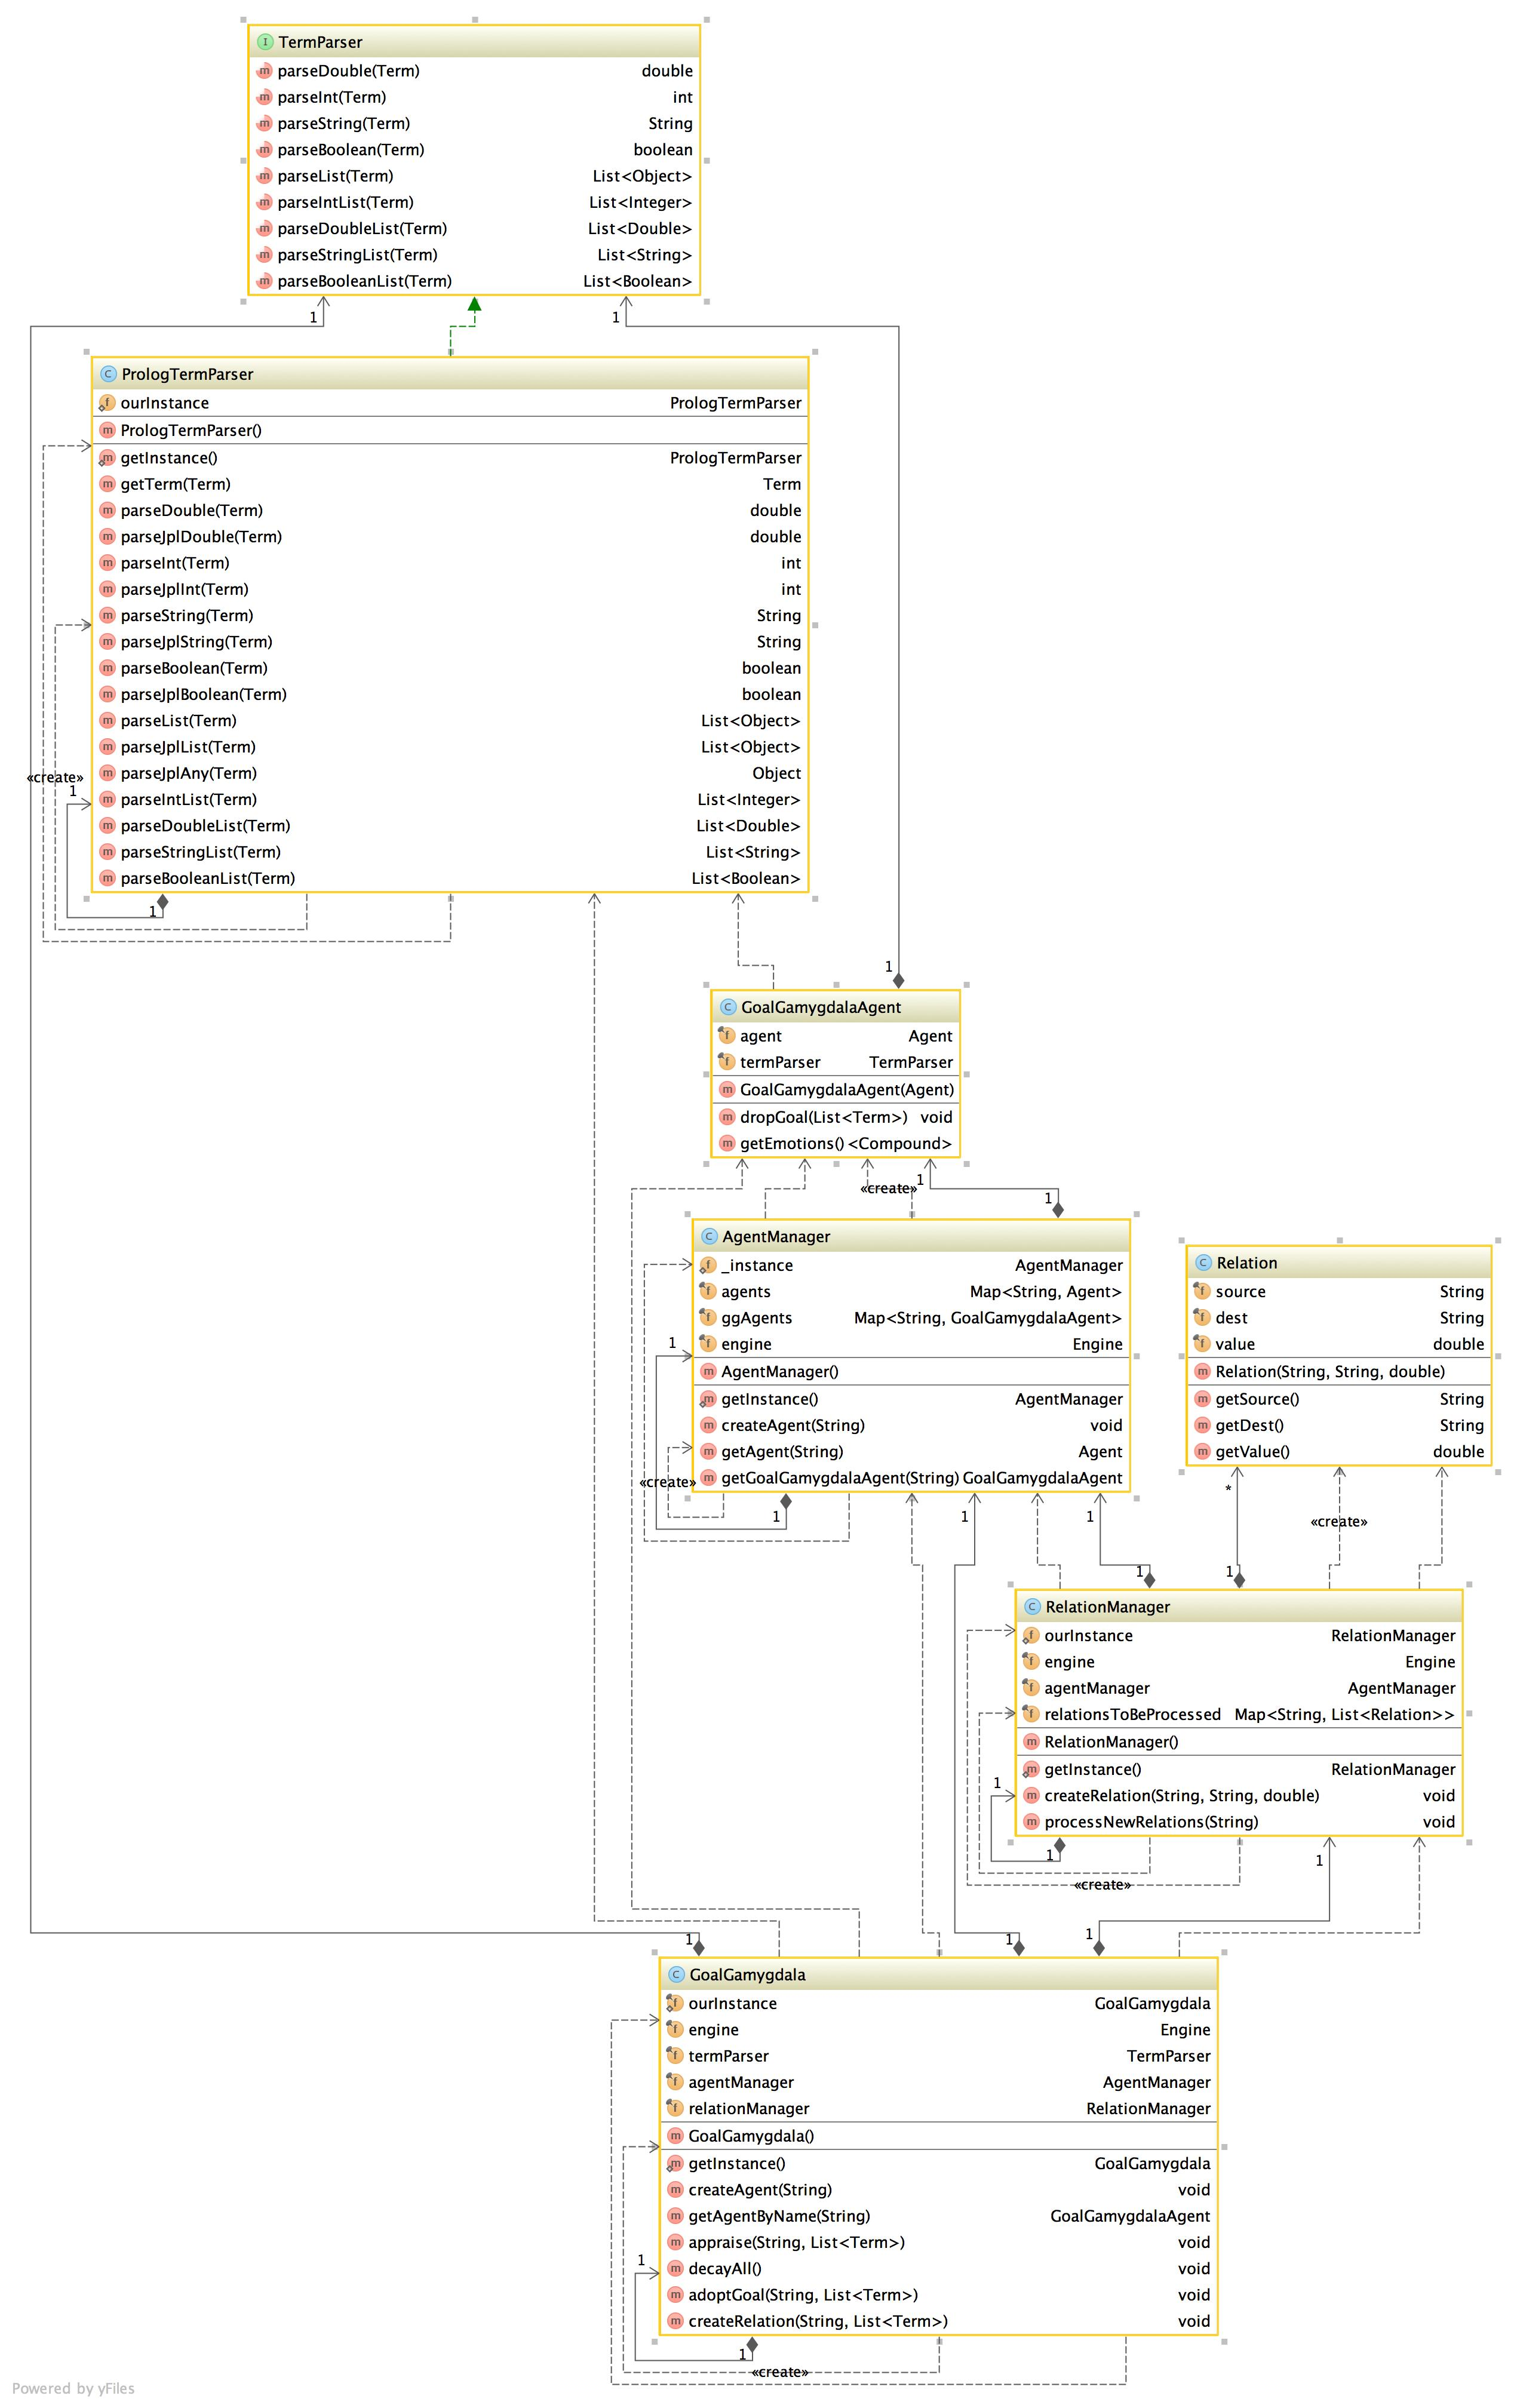
\includegraphics[width=\linewidth]{diagram-goalgamygdala}
\caption{The UML-diagram for the GOAL-GAMYGDALA interface.}
\end{figure}